\documentclass[twoside,11pt]{article}

%================================ PREAMBLE ==================================

%--------- Packages -----------
\usepackage{fullpage}
\usepackage{amssymb}
\usepackage{amsmath}
\usepackage{amsthm}
\usepackage{latexsym}
\usepackage{graphicx}
\usepackage{wrapfig}
\usepackage{color}
\usepackage{url}
\usepackage{float}
\usepackage{enumitem}
\usepackage{wrapfig}
\usepackage{titlesec}
%\usepackage{algorithm,algorithmic}

%---------- Spacing ----------
\setlength{\parindent}{0pt}
\setlength{\parskip}{3pt}

\setlist[enumerate]{itemsep=0mm}
\titlespacing*{\section}{0pt}{0.6\baselineskip}{\baselineskip}

%---------Definitions----------
\newcommand{\half}{{\textstyle{\frac{1}{2}}}}
\renewcommand{\>}{{\rightarrow}}
\renewcommand{\hat}{\widehat}
\renewcommand{\tilde}{\widetilde}
\newcommand{\grad}{{\nabla}}
%
\newcommand{\argmax}{\textup{\textrm{argmax}}}
\newcommand{\argmin}{\textup{\textrm{argmin}}}
\newcommand{\argsort}{\textup{\textrm{argsort}}}
\newcommand{\sign}{\textup{\textrm{sign}}}
\newcommand{\poly}{\textup{\textrm{poly}}}
\newcommand{\er}{\textup{\textrm{er}}}
\newcommand{\zo}{\textup{\textrm{0-1}}}
\newcommand{\sq}{\textup{\textrm{sq}}}
%
\newcommand{\1}{{\mathbf 1}}
\newcommand{\0}{{\mathbf 0}}
\newcommand{\I}{{\mathbf I}}
\newcommand{\R}{{\mathbb R}}
\newcommand{\Z}{{\mathbb Z}}
\newcommand{\N}{{\mathbb N}}
\renewcommand{\P}{{\mathbf P}}
\newcommand{\E}{{\mathbf E}}
\newcommand{\Var}{{\mathbf{Var}}}
%
\renewcommand{\a}{{\mathbf a}}
\renewcommand{\b}{{\mathbf b}}
\renewcommand{\c}{{\mathbf c}}
\renewcommand{\d}{{\mathbf d}}
\newcommand{\f}{{\mathbf f}}
\renewcommand{\k}{{\mathbf k}}
\newcommand{\p}{{\mathbf p}}
\newcommand{\q}{{\mathbf q}}
\renewcommand{\u}{{\mathbf u}}
\newcommand{\w}{{\mathbf w}}
\newcommand{\x}{{\mathbf x}}
\newcommand{\y}{{\mathbf y}}
%
\newcommand{\A}{{\mathbf A}}
\newcommand{\bC}{{\mathbf C}}
\newcommand{\C}{{\mathcal C}}
\newcommand{\cD}{{\mathcal D}}
\newcommand{\F}{{\mathcal F}}
\renewcommand{\H}{{\mathcal H}}
\newcommand{\K}{{\mathbf K}}
\renewcommand{\L}{{\mathcal L}}
\newcommand{\bL}{{\mathbf L}}
\newcommand{\cN}{{\mathcal N}}
\newcommand{\W}{{\mathbf W}}
\newcommand{\X}{{\mathcal X}}
\newcommand{\bX}{{\mathbf X}}
\newcommand{\Y}{{\mathcal Y}}
%
\newcommand{\bloss}{{\boldsymbol \ell}}
\newcommand{\blambda}{{\boldsymbol \lambda}}
\newcommand{\bmu}{{\boldsymbol \mu}}
\newcommand{\bnu}{{\boldsymbol \nu}}
\newcommand{\bSigma}{{\boldsymbol \Sigma}}
\newcommand{\seta}{{\boldsymbol \eta}}
\newcommand{\bpsi}{{\boldsymbol \psi}}
\newcommand{\bphi}{{\boldsymbol \phi}}
\newcommand{\bPhi}{{\boldsymbol \Phi}}
\newcommand{\balpha}{{\boldsymbol \alpha}}
\newcommand{\bxi}{{\boldsymbol \xi}}

%=============================== END PREAMBLE ===============================

\begin{document}

%================================ COVER PAGE ================================

%*********** Use this for project proposal (comment out in project report) ************
\emph{\footnotesize{CIS 520 Spring 2018, Project Proposal}}

%*********** Use this for project report (comment out in project proposal) ************
%\emph{\footnotesize{CIS 520 Spring 2018, Project Report}}

\vspace{12pt}

%Fill in your project title
\textbf{\Large{Word Sense Disambiguation by Supervised Learning}}

\vspace{1cm}

\textbf{Team Members:}

%Fill in your team details; remove any lines that are not needed
Haoxian Chen (PennKey: \texttt{hxchen}; Email: \texttt{hxchen@seas.upenn.edu}) \\
Leshang Chen (PennKey: \texttt{leshangc}; Email: \texttt{leshangc@seas.upenn.edu}) \\
Hui Lyu (PennKey: \texttt{huilyu}; Email: \texttt{huilyu@seas.upenn.edu}) \\
Yanci Zhang (PennKey: \texttt{yanci}; Email: \texttt{yanci@seas.upenn.edu})

%---

\vspace{2cm}

%*********** Comment out the following for the proposal; uncomment and fill in all details for the project report ***********

\textbf{Assigned Project Mentor:}

%Fill in assigned TA name
TA-Firstname TA-Lastname

\vspace{1cm}

\textbf{Team Member Contributions:}

%Fill in team member contributions
\begin{center}
\begin{tabular}{|l|l|}
\hline
Team Member & Contributions \\
\hline
Firstname1 Lastname1 & list of contributions \\
	& (continue if needed) \\
\hline
Firstname2 Lastname2 & list of contributions \\
	& (continue if needed) \\
\hline
Firstname3 Lastname3 & list of contributions \\
	& (continue if needed) \\
\hline
Firstname4 Lastname4 & list of contributions \\
	& (continue if needed) \\
\hline
\end{tabular}
\end{center}

\vspace{12pt}

\textbf{Code Submission:}

[Mention whether code is being submitted on Canvas or via a github repository; if latter, provide a link to the repository]


\newpage
%============================= MAIN DOCUMENT ================================

%*********** Use this to include abstract in project report (comment out in project proposal) ***********
%\begin{abstract}
%Abstract for project report goes here.
%\end{abstract}


%*********** Recommended section structure for project proposal below (comment out in project report) ************

\section{Introduction}

\begin{wrapfigure}{l}{0.5\textwidth}\centering
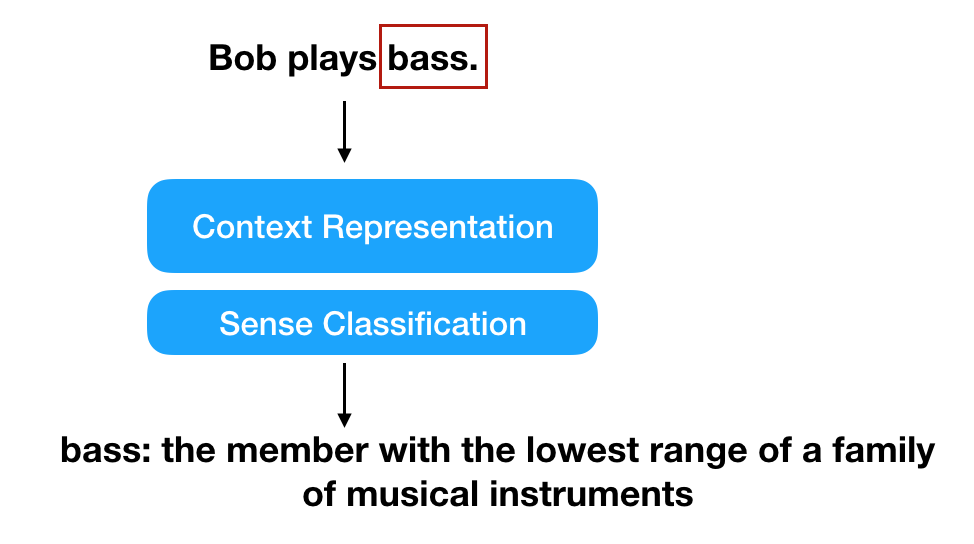
\includegraphics[width=0.5\textwidth]{graphs/overview.png}
\caption{system overview}
  \label{fig:overview}
\end{wrapfigure}

Words in natural language could have multiple meanings. Though humans are good
at inducing the actual meaning of words given a certain context, such
multi-meaning words are often seem ambiguous to machines. Such ambiguiaty in
natural languages have been the major challenges for machine to understand user
intention, e.g. google search key words.

To solve this problem, we propose to build a word sense disambiguate system that
takes an English word and a sentence where it appears as input, and predicts the
sense of such word within the given context. 
The architecture of our system is shown in figure~\ref{fig:overview}.


\section{Related Work}

Major approaches to the word sense disambiguation problem can be briefly
categorized into three types: Knowledge-based, supervised learning, and
unsupervised learning. 

Knowledge based appraoch.
Lesk's algorithm~\cite{lesk1986automatic} is a
dictionary-based approach. It assumes that words appear within the same context
have related semantics. The alogrithm disambiguate word sense by finding the
dictionary definition that shares the most common words with the given context
sentence.

Supervised learning approaches. These approaches typically use a hand-annotated
Corpus as the training data set. The classifier is concerned on each individual
word, and the output is one of the definition of the ambiguous word in the
dictionary. Over the decades, people have proposed different algorithms to solve
this classification problem: decision-tree~\cite{quinlan1986induction}, 
Naive Bayers classifier~\cite{ng1997getting}, Neural
Network~\cite{cottrell1985connectionist}, and SVM~\cite{lee2002empirical}, etc.

Unsupervised approach. Such approaches~\cite{schutze1998automatic} assumes that
similar senses appear in similar contexts. By clustering occurrance of words
into clusters using some similarity measures, the sense of a new occurring word
can be induced by assigning it to the closest cluster.

% \textbf{Context representation.} To feed sentences into our system, we need to
% encode the context into some data structure. Previous researches have proposed
% several ways to represent context.


\section{Problem formulation}

This is a supervised multi-class classification problem. For each targetted
ambiguous word $w$, we train an classifier $h_w: X \rightarrow L$, where X is
the feature space (context representation), and the label space L is the list of
word definitions for word w given by WordNet~\cite{wordnet}.

\textbf{Data Preprocessing}.

We plan to use SemCor Corpus~\cite{semcor} as our data set. SemCor Corpus is a
corpus where each word is tagged with a sense provided by WordNet~\cite{wordnet}.

\begin{enumerate}
  \item Tokenization: transform the sentense strings into list of tokens
    (usually words).
  \item Part-of-Speech tagging: e.g. ``the/DT bar/NN was/VBD crowded/JJ'', where
    DT stands for Determiners, NN stands for Noun, etc.
  \item Lemmatization: e.g. $plays \rightarrow play$, $was \rightarrow be$.
  \item Feature extraction: select some features to represent the context.
\end{enumerate}

Feature extraction (context representation): 
(1) Colocation~\cite{colocation}. The preceding and succeeding words and their
Part-of-Speech tags.  (2) Bag-of-words~\cite{bagofwords}. Ignore positional
information. Assume that there is a fixed set of vocabulary that represent a
relevant topic, transform the appearance of those words as a bit vector.

\textbf{Construct training set for each target word}.\\
Let W be the set of English words that we want to do sense disambiguation. For
each $w \in W$, we need to extract a training set $X_w$ from the SemCor Corpus
as follow: 
\begin{enumerate}
  \item Draw a set of sentences $S_w$ from SemCor Corpus, where each 
$s \in S_w$ contains w. 
  \item Convert each sentence $s \in S_w$ to a feature vector x, and the sense
    label y. The set of all (x,y) pairs is our training set $X_w$.
\end{enumerate}



\section{Solution Methods}

For this multi-class classification problem, we consider the following models,
using one-vs-all method to extend them to solve multi-class problem:
\begin{itemize}
  \item Naive Bayes.
  \item Logistic Regression.
  \item Support Vector Machine.
  \item Neural Networks.
\end{itemize}

\textbf{Desired properties}. Since in our system design, we need to train a
classifier for each target word, the ideal method should have short training
time, and compact model representation.

\textbf{Performance Measure}. For each target word, we partition the data into
training set and test set. And evaluate classifiers on the training set using
0-1 loss.


\section{Plan of Work}
\begin{itemize}
  \item Week 1: Data preprocessing. 
      Tokenization: Haoxian Chen.
      Part-of-Speech tagging: Leshang Chen.
      Lemmatization: Hui Lyu.
      Feature extraction: Yanci Zhang.
  \item Week 2: Algorithm implementations.
      Naive Bayes: Haoxian Chen.
      Logistic Regression: Leshang Chen.
      Support Vector Machine: Hui Lyu.
      Nueral Network: Yanci Zhang.
  \item Week 3: Performance comparison and analysis. 
  \item Week 4: Report Writing.
\end{itemize}


% \section*{Acknowledgments}

%*********** Recommended section structure for project report below (comment out in project proposal) ************

%\section{Introduction}

%\section{Related Work}

%Note: Using BibTex makes it easy to include citations to references! For example, here are citations to Bishop's book \cite{Bishop06}, the UCI machine learning repository \cite{DuaKa17}, and a couple of papers \cite{FreundSc96,LeCun+15}.

%\section{Data Set}

%\section{Problem Formulation}

%\section{Algorithms}

%\section{Experimental Design and Results}

%\section{Conclusion and Discussion}

%\section*{Acknowledgments}


\newpage
%============================= BIBLIOGRAPHY ===============================

\bibliographystyle{unsrt}
\bibliography{bib}

\end{document}

%=========================== END DOCUMENT ==============================

